\newpage
\begin{center}
	\textbf{\large ГЛАВА 5}

	\textbf{\large НЕЙРОННЫЕ СЕТИ В ЗАДАЧЕ ПРЕДСКАЗАНИЯ ВЗАИМОДЕЙСТВИЯ БЕЛКОВ}
\end{center}
\refstepcounter{chapter}
\addcontentsline{toc}{chapter}{5. НЕЙРОННЫЕ СЕТИ В ЗАДАЧЕ ПРЕДСКАЗАНИЯ ВЗАИМОДЕЙСТВИЯ БЕЛКОВ}

В данной главе описаны нейронные сети, использованные и предлагаемые к использованию для решения задачи предсказания взаимодействия белков, а также подходы к процессу обучения таких сетей. Основные фокусы при проектировании таких сетей:
\begin{itemize}
\item Использование матриц косинусов для представления входных/выходных данных;
\item Применимость к данным различных размеров.
\end{itemize}

\section{Архитектура нейронных сетей}

\subsection{Полносвёрточная нейронная сеть FCN5}
Полносвёрточнная нейронная сеть\cite{fully_conv} -- это свёрточная нейронная сеть, в которой отсутствуют полносвязные слои. Как и все свёрточные сети, полносвёрточные сети позволяют эффективно обрабатывать изображения различных размерностей, наиболее часто - двумерных. Главной особенностью свёрточнных сетей без полносвязных слоёв является то, что они могут преобразовывать входные изображения практически любых размеров без масштабирования. Это крайне важное свойство при работе с матрицами косинусов, так как в отличие от графических изображений, их нельзя масштабировать. В рамках данной работы использовалась сеть FCN5, которая была разработана и использована еще в \cite{prip2023}. Несколько сетей FCN5 можно последовательно объединнить в одну большую, если это необходимо.

Сеть FCN5 состоит из 5 остаточных слоёв \cite{resnet}, 2 слоёв батч-нормализации \cite{batchnorm}, между слоями присутствуют \textit{пропускные связи}.

Используемые остаточные слои задаются количеством входных и выходных каналов, состоят из двух свёрточных слоёв, и организованы следующим образом:
\begin{enumerate}
\item Входной тензор поступает на первый свёрточный слой, который производит промежуточный тензор. Количество каналов в промежуточном тензоре равно количеству выходных канналов.
\item К промежуточный тензору применется функция активации ReLU, а результат поступает на выход второго свёрточного слоя. Второй свёрточный слой сохраняет количесвто каналов тензора.
Выход второго свёрточного слоя суммируется с промежуточным тензором (до применения ReLU), а к результату применяется функция активации LeakyReLU с параметром отрицательного склона равного 0,2 (функия активации не применняется для последнего остаточного блока в сети). Полученный тензор является выходом остаточного слоя.
\item Размер ядра используемых свёрток -- $3\times3$.
\item Для сохранения размеров (ширины и высоты) входных тензоров используется круговой паддинг. Использование других видов паддинга (нулевого, зеркального) не рекомендуется.
\end{enumerate}

Смысл пропускных связей (англ. \textit{skip connection}) заключается в том, чтобы отправлять на вход слоя нейронной сети не просто выход предыдущего слоя, но выход предыдущего слоя соединённый (коннкатенация каналов) с выходами еще более ранних слоёв. Общее устройство сети FCN5 можно увидеть на следующей схеме:
\begin{figure}[H]
	\centering
	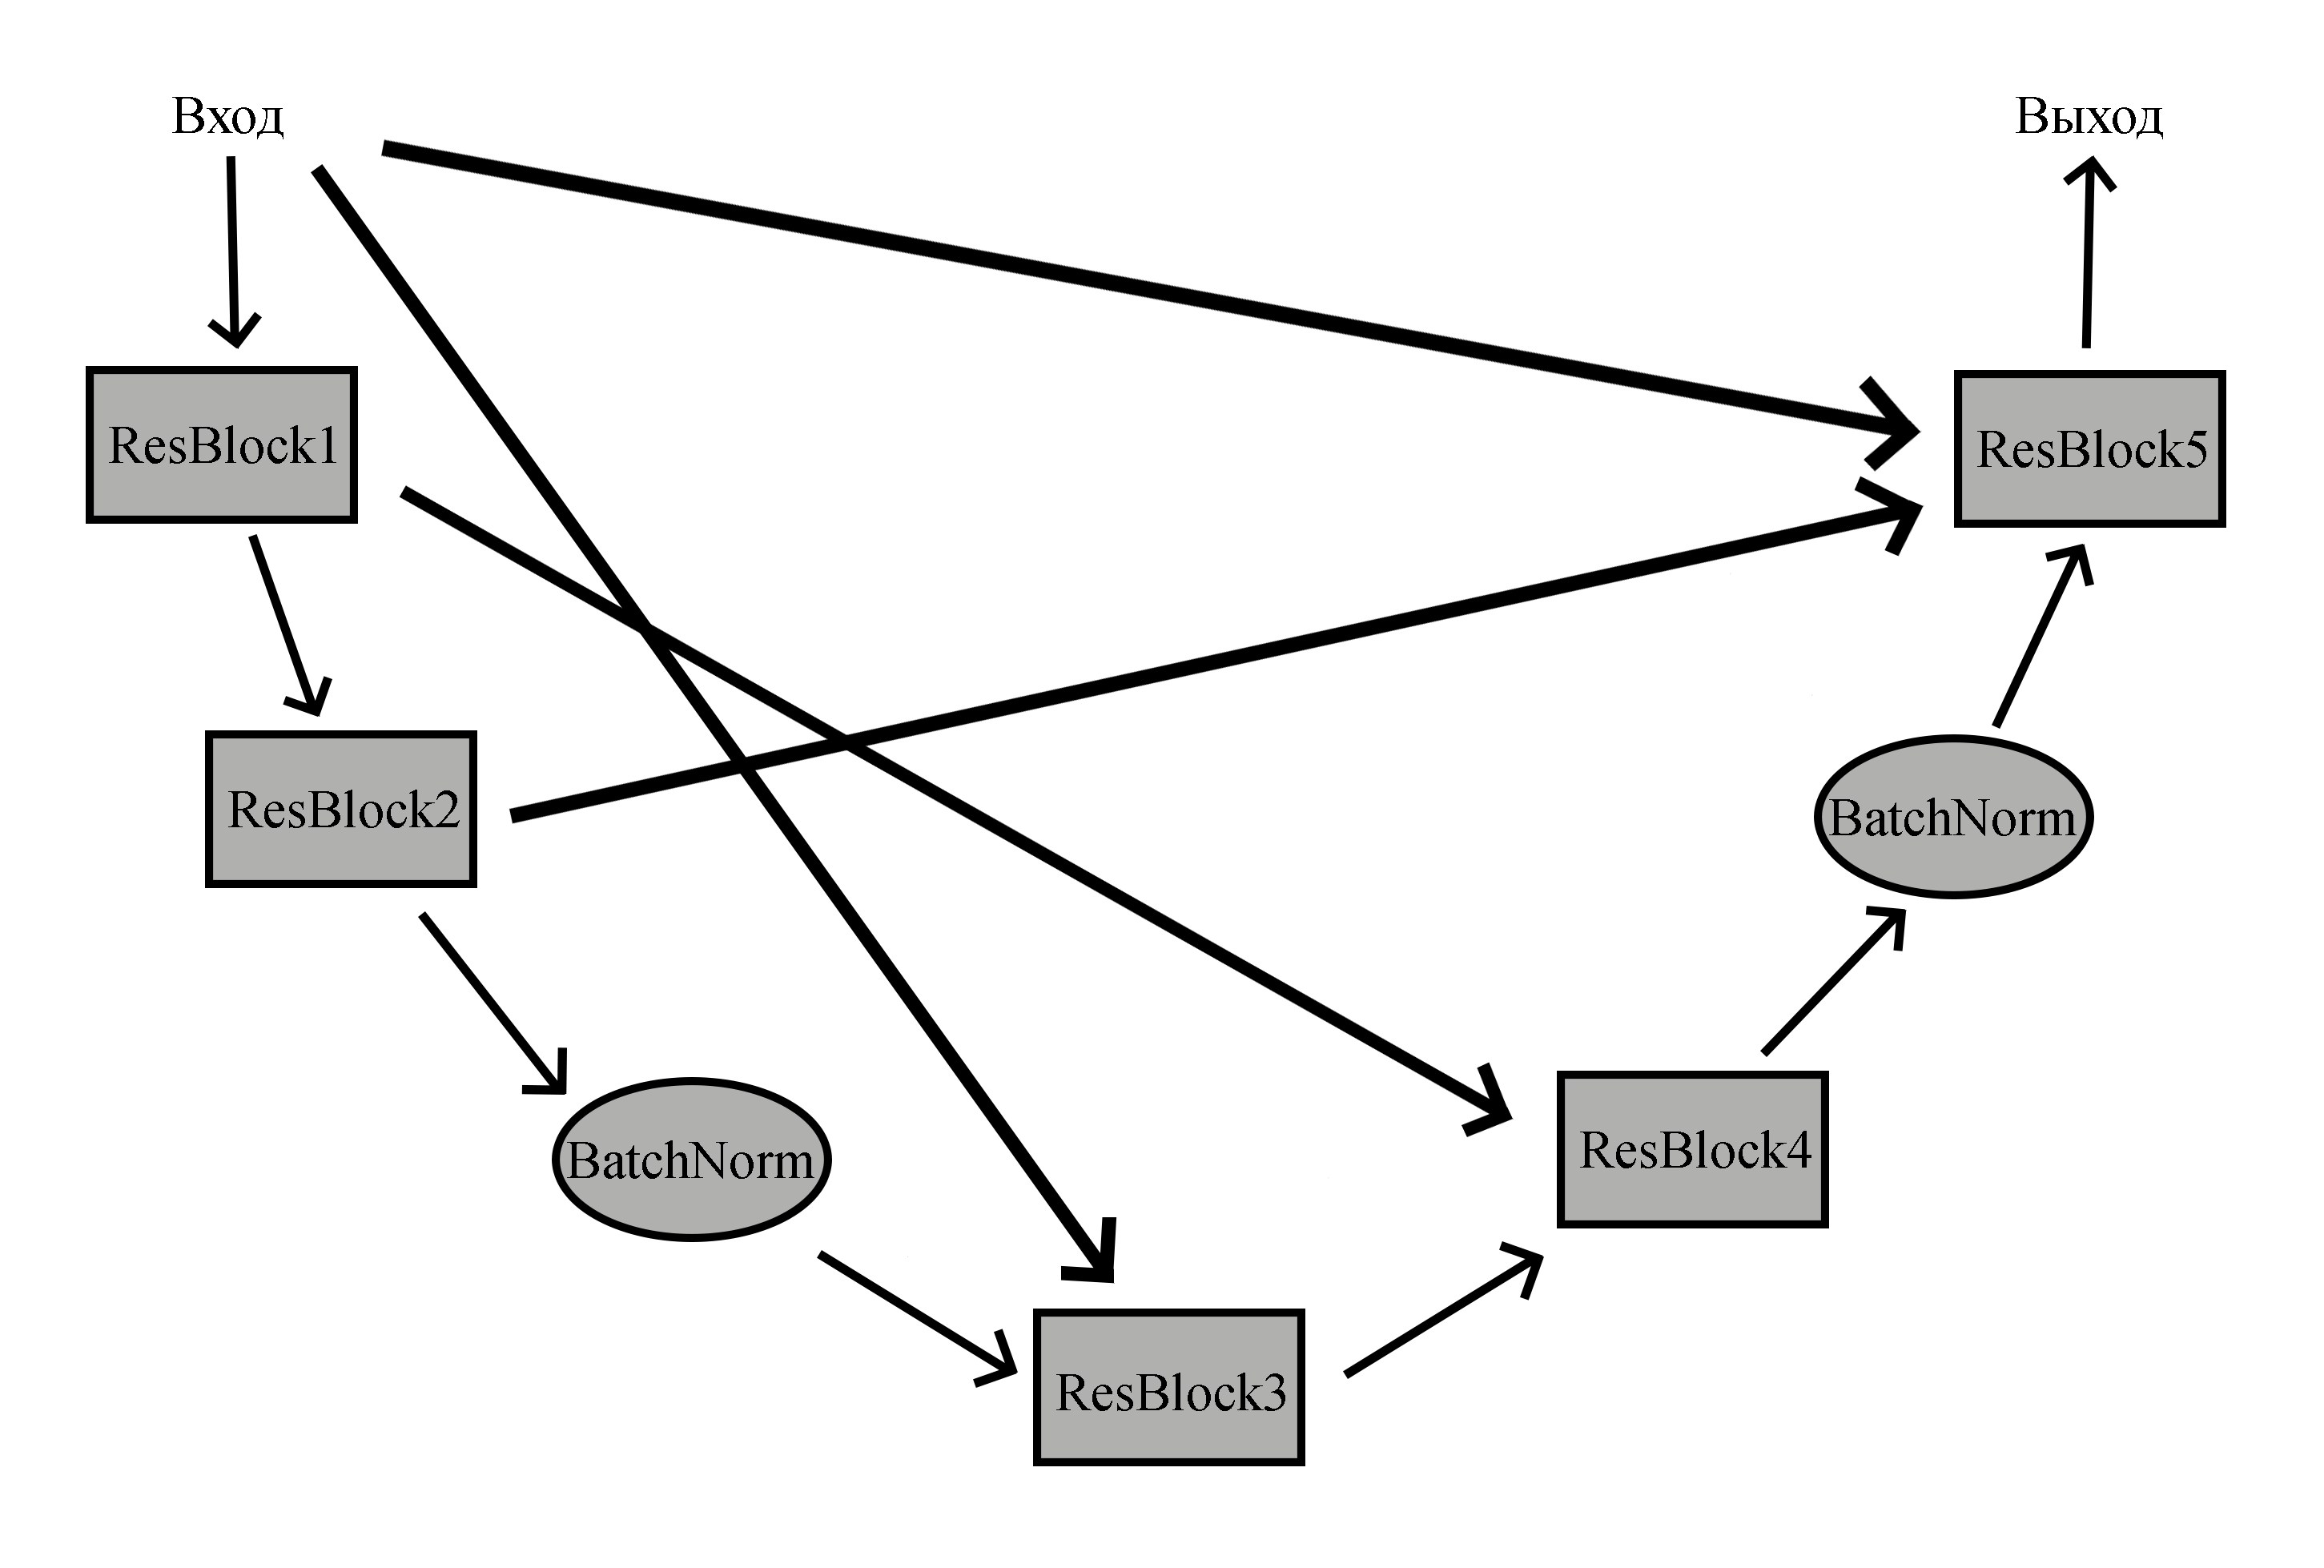
\includegraphics[width=\textwidth]{FCN5.png}
	\caption{Устройство сети FCN5.}
	\label{fig_fcn5}
\end{figure}

Сеть FCN5 по устройству крайне близка к сетям типа U-Net\cite{unet}. Но сеть U-Net известна тем, что количество каналов промежуточных тензоров сначала растёт, а потом убывает. При работе с FCN5, как и в большинстве других свёрточных сетей, количество каналов растёт от начала до конца.

Отметим, что количество каналов входного, а также количество выходных каналов в 5 остаточных слоях могут быть произвольными. В экспериментах часто использовалась следующая комбинация для промежуточных слоёв (входные каналы и пятый слой зависят от типа данных):
\begin{itemize}
\item Остаточный слой 1: 128 каналов;
\item Остаточный слой 2: 256 каналов;
\item Остаточный слой 3: 512 каналов;
\item Остаточный слой 4: 256, 384 или 512 каналов.
\end{itemize}
Для ускорения вычислений, также можно использовать уменьшенный вариант:
\begin{itemize}
\item Остаточный слой 1: 32 канала;
\item Остаточный слой 2: 64 канала;
\item Остаточный слой 3: 128 каналов;
\item Остаточный слой 4: 43 канала.
\end{itemize}

\subsection{Концепция сети-трансформера}
Основным недостатком полносвёрточных нейронных сетей является то, хоть они и могут обрабатывать изображения сколь угодно больших размеров (на сколько то позволяет память компьютера), для изображений крайне малого размера (которые в рамках данного исследования могут возникнуть при работе с пептидами), может оказаться, что применяемых свёрток слишком много (каждая свёртка уменьшает размер изображения, после чего операция паддинга возвращает исходный размер), и результат окажется совершенно ненадёжным. Также отметим, что операция свёртки локальна -- за формирования одного пикселя выходнного изображения отвечает ограниченная область вокруг этого пикселя в исходнном изображении. Это значит, что практически отстутствует связь между удалёнными участками изображения.

Наиболее привлекательным решением таких проблем выглядит использование сети-трансформера\cite{attention_all_you_need}. Такие сети в настоящее время получили крайне широкое распространение, прежде всего в задачах обработки естественного языка, но также и в задачах биоинформатики. Сети-трансформеры хорошо работают с данными, представленными в виде последовательностей, позволяют эффективно находить связи между удалёнными участками таких последовательностей.

Концептуально, в такой сети можно использовать токен, бинарнно кодирующий 5 аминокислотных остатков и релятивистскую матрицу косинусов размера $4\times4$. На выходе можно, например, получать токены с матрицами косинусов $4\times4$, кодирующими матричное поле. Можно использовать и более простые выходные токены.

\section{Представление данных и процесс обучения нейронной сети}

\subsection{Набор данных}

Для создания набора данных использовались записи из банка данных PDB, загруженнные ранее 31 октября 2022. Была составлена программа, которая выявляла среди этих файлов модели белковых комплексов.
% 2-mer: 24370
% 3-mer: 4212
% 4-mer: 7987
% 5-mer: 732
% 6-mer: 2335
% 7-mer: 164
% 8-mer: 1270
% high-mer: 1853
Было обнаружено:
\begin{itemize}
\item 24370 димерных комплексов;
\item 4212 тримерных комплексов;
\item 7987 4-мерных комплексов;
\item 732 5-мерных комплексов;
\item 2335 6-мерных комплексов;
\item 164 7-мерных комплексов;
\item 1270 8-мерных комплексов;
\item 1853 комплексов более высокого порядка.
\end{itemize}
% train: 19496
% valid: 4874

После фильтрации, которая включала в себя выделение всех попарных взаимодействий, исключая содержащие нестандартные аминоксилотные остатки, а также слишком короткие взаимодействующие молекулы, получили наборы данных из:
\begin{itemize}
\item 85014 взаимодействий в обучающем наборе; 
\item 21547 взаимодействий в тестовом наборе.
\end{itemize}
% train items: 85014
% valid items: 21547
% Oct 31 2022

\subsection{Процесс обучения}
Нейронная сеть обучается в течении нескольких больших итераций, называемых эпохами. Одна эпоха означает один полный обход тестового набора данных, и валидацию на всём тестовом наборе. Каждую эпоху делят на некоторое число итераций, при которых выделяется фиксированный <<кусок>> тестового набора данных (батч), который обрабатывается нейронной сетью, результат оценивается с помощью некоторой функции потерь, после чего веса нейрронной сети обновляются для минимизации этой самой функции потерь. Валидация тестового набора данных также производится по батчам.

В предлагаемом подходе, типичная итерация обучения выглядит следующим образом: 
\begin{enumerate}
\item Из набора данных выбирается следующий батч. Для этого в каждой записи о взаимодействии двух молекул выбирают пару взаимодействующих остатков, и производят обрезку обеих молекул под фиксированный размер так, чтобы взаимодействующая пара остатков сохранилась. Теперь, для сравнения, либо выбирают точку, где взаимодействия нет (для \ref{L_multiscalar}), либо строят другую, ложную модель взаимодействия. Координаты, закодированные аминокислотные остатки, а также координаты точек взаимодействия собирают в тензоры и отправляют на память видеокарты.
\item На видеокарте из координат атомов и точек взаимодействия строят соответствующую релятивистскую матрицу косинусов. Код аминокислотных остатков дополнительно обрабатывают, и записывают в виде матрицы.
\item Нейросеть высчитывает матрицы косинусов, кодирующие обобщённые переменные поля для истинного и ложного взаимодействия. Из этих матриц извлекают эти переменные и высчитывают частичные лагранжианы $L^{T}_{part}$ и $L^{F}_{part}$. 
\item В качестве функции потерь проще всего использовать разницу $L^{T}_{part} - L^{F}_{part}$, что будет приводить к тому, что истинным моделям будет сопоставляться меньший частичный лагранжиан, чем ложным. Также желательно, чтобы выполнялось: $L^T_{part} < 0$ и $L^{F}_{part} > 0$, для чего использовалась функция потерь:
\begin{equation}
	l(L^{T}_{part}, L^{F}_{part}) = \frac{(L^{T}_{part} - L^{F}_{part}) - \relu(-L^{T}_{part}) + \relu(-L^{F}_{part})}{2}.
	\label{loss_function}
\end{equation}
К данной функции также можно добавить значение (с маленьким весом), которое отражающую внутреннюю согласованность предсказанной матрицы косинусов (для этого из матрицы сначала получают обобщённые переменные, а потом по этим переменным опять строят матрицу, после чего считаеют разницу между первым и вторым).
\item Посчитанная $l(L^{T}_{part}, L^{F}_{part})$ минимизируется методом оптимизации Adam.
\end{enumerate}
\begin{figure}[H]
	\centering
	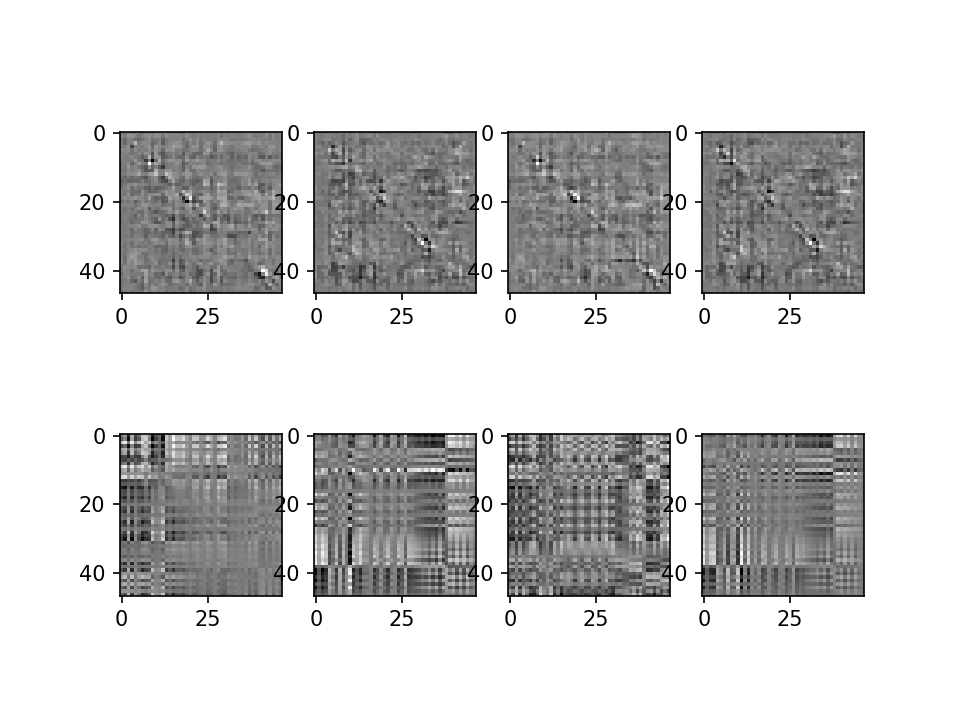
\includegraphics[width=\textwidth]{a5.png}
	\caption{Пример малой согласованности матриц. Верхняя строка -- выход нейронной сети, нижняя -- вид корректных матриц.}
	\label{fig_consistency}
\end{figure}

В следующей главе изложены результаты использования описанного выше подхода.
